\subsection{Redes Inalámbricas}
Una red inalámbrica es un sistema de comunicación de datos flexible que reduce la necesidad de conexiones físicas al enviar y recibir datos por aire a través de medios inalámbricos, como la tecnología de radiofrecuencia. Las redes de datos están experimentando un cambio significativo gracias a la revolución de las comunicaciones inalámbricas. Los recientes avances en las redes y la tecnología inalámbrica han permitido que la gran mayoría de los dispositivos inalámbricos que se utilizan hoy en día se conecten fácilmente. Es necesario maximizar el uso de los recursos del espectro para permitir que millones de dispositivos inalámbricos se conecten inalámbricamente. \parencite{tec_pundalik2023anwirnet}

Las redes inalámbricas utilizan ondas electromagnéticas para transferir información entre lugares sin tener conexiones físicas. Las ondas de radio suelen denominarse portadoras de radio, ya que sólo envían energía a un receptor distante. Los datos que se transfieren se superponen a la onda de radio para garantizar una extracción precisa en el extremo receptor. Debido a que la frecuencia de la información de modulación o la velocidad de bits se suman a la portadora de radio después de que los datos se superponen (modulan) sobre ella, la señal de radio tiene muchas frecuencias. Si las ondas de radio se envían en diferentes frecuencias de radio, varias portadoras de radio pueden coexistir en el mismo espacio sin interferir entre sí. Las señales de radio, los formatos de datos y la arquitectura de la red son los tres componentes de una red inalámbrica. Dado que estos tres elementos no están relacionados entre sí, deben describirse al construir una nueva red. Mientras que la señal de radio opera en la capa física, el formato de datos tiene un impacto en varios niveles superiores del modelo de referencia OSI. Las estaciones base y los adaptadores de interfaz de red inalámbrica son componentes de la estructura de la red que envían y reciben señales de radio. Cada computadora y estación base en una red inalámbrica tiene adaptadores de interfaz de red que transforman los datos digitales en señales de radio, que luego se envían a otros dispositivos conectados. Además, reciben y transforman las señales de radio entrantes de otros componentes de la red en datos digitales. Los formatos de datos, las arquitecturas de red y las señales de radio son distintos para cada servicio de datos inalámbricos de banda ancha. \parencite{tec_rafaqat2019surveywir}

Las redes inalámbricas se clasifican normalmente en cinco grupos distintos. La región de aplicación y el rango de señal son los principales criterios utilizados para esta clasificación (Figura 30). Las redes inalámbricas en el primer grupo, WBAN, conectan dispositivos en la superficie del cuerpo entre sí. Las señales de estas redes pueden alcanzar un máximo de dos metros. El segundo grupo, conocido como WPAN, está compuesto por redes inalámbricas con un alcance de señal mínimo de 10 metros que se utilizan para conectar varios dispositivos entre sí. El tercer grupo cumple con el estándar de redes inalámbricas, que busca cubrir un edificio o habitación como máximo. El alcance de señal de este grupo, conocido como WLAN, suele ser de 30 metros en interiores y de 100 a 200 metros en exteriores. El término fidelidad inalámbrica (Wi-Fi o IEEE 802.11) se usa con frecuencia para describir la tecnología inalámbrica. La WMAN, la cuarta clase de red inalámbrica, permite a los usuarios conectarse a Internet con un alcance de señal de entre 5 y 20 kilómetros. Este protocolo a menudo se conoce como IEEE 802.16-2001, también conocido como interoperabilidad mundial para acceso por microondas (WiMAX). El WWAN es el grupo final. Las redes WWAN (redes basadas en GSM y CDMA) ofrecen conexiones inalámbricas en una área mucho más amplia que el grupo anteriormente mencionado utilizando la infraestructura de red de los operadores móviles. \parencite{tec_ieee2010draft}
\begin{figure}[!ht]
	\begin{center}
		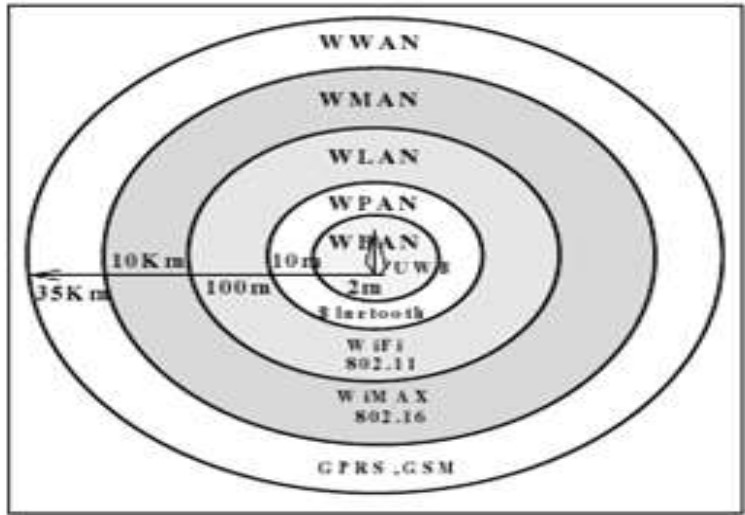
\includegraphics[width=0.85\textwidth]{2/figures/clasificacionredes.jpg}
		\caption[Clasificación de redes inalámbricas con su alcance de señal]{Clasificación de redes inalámbricas con su alcance de señal.\\
			Fuente: \cite{tec_ieee2010draft}. \citetitle{tec_ieee2010draft}.}
		\label{2:fig52}
	\end{center}
\end{figure}

\subsection{Calidad de Servicio (QoS)}
La expansión de las redes de datos de alta velocidad depende de la calidad de servicio (QoS). Esto es particularmente cierto cuando se trata de cumplir con las limitaciones de velocidad de datos y latencia de paquetes de los consumidores de datos en tiempo real. Al transferir un flujo de paquetes desde el origen al destino, la red debe cumplir con ciertos requisitos de calidad de servicio (QoS). Debido a este requisito, las redes que utilizan comunicación inalámbrica enfrentan desafíos especiales. La calidad de un canal inalámbrico varía significativamente entre los usuarios y cambia enormemente con el tiempo, tanto en escalas de tiempo lentas como rápidas. Además, el ancho de banda inalámbrico generalmente es limitado y debe utilizarse con precaución. Encontrar formas eficientes de proporcionar QoS para datos en tiempo real (como transmisiones de audio y video en vivo) a través de canales inalámbricos es necesario para brindar la calidad de servicio (QoS) adecuada a la mayor cantidad de personas posible \parencite{tec_pang2010wifireport}. La confiabilidad de la red siempre ha sido crucial para muchas aplicaciones de red. Sin embargo, con el aumento en la cantidad de datos de audio y video que se transmiten a través de las redes abiertas de conmutación de paquetes, la capacidad de garantizar la calidad de servicio (QoS) en las redes actuales puede ser más crucial que nunca. Como resultado, se ha dedicado una gran cantidad de tiempo y esfuerzo a encontrar una forma de mantener un rendimiento constante de la red mientras se utilizan todos los recursos disponibles. Las garantías de servicio probablemente sean el requisito previo más importante para el éxito de la transmisión de audio y video. Muchos proveedores de servicios han comenzado a utilizar redes de conmutación de paquetes para ofrecer servicios de video y telefonía en los últimos años. Una de las razones por las que se crearon estos servicios es que la red IP ofrece capacidad adicional que puede utilizarse por una fracción del costo de una red dedicada de conmutación de circuitos. Otro argumento es que la naturaleza libre de forma de una red de conmutación de paquetes aumenta su adaptabilidad y permite la creación de nuevos servicios como video bajo demanda. Los diferentes métodos de compresión codifican los flujos a diferentes velocidades de bits para maximizar la eficiencia, lo que crea un problema único para la transmisión de audio/vídeo (VBR). Es posible garantizar el rendimiento a tasas de bits más altas para tales flujos, pero esto es ineficaz. Un sistema de calidad de servicio (QoS) mejorado también garantizaría el rendimiento a la velocidad de bits promedio y permitiría el tráfico en ráfagas con la menor pérdida y retraso. \parencite{tec_pang2010wifireport}

\subsection{Diferentes parámetros que deben enviarse para las comunicaciones de extremo a extremo a través de redes inalámbricas }

Actualmente, la información se presenta en una variedad de formatos, como texto, imágenes, sonido y video.

\begin{itemize}
	\item \textbf{Textos}: En tecnología de la información, el texto es una serie de caracteres que los humanos pueden leer y luego codificar en formatos legibles por computadora como ASCII. Las imágenes visuales en forma de mapas de bits, que en realidad están en su propio formato legible por computadora, y el código de programa, al que con frecuencia se hace referencia como "binario", son ejemplos de datos que no han sido codificados con caracteres. En las transmisiones de datos, el texto se representa como una serie de bits o un patrón de bits (0 o 1). Muchos conjuntos de patrones de bits se han desarrollado para representar símbolos de texto. El proceso de representar símbolos se conoce como codificación, y cada conjunto se denomina código. El sistema de codificación popular actual, Unicode, representa cada letra o símbolo en cualquier idioma del mundo en 32 bits. El Código Estándar Americano para el Intercambio de Información (ASCII), creado hace muchos años en los Estados Unidos, es responsable de los primeros 127 caracteres de Unicode, que se conocen comúnmente como Latín Básico. \parencite{tec_marks2001standieee}
	\item \textbf{Imágenes}: Las imágenes también se pueden representar utilizando patrones de bits. Una matriz de píxeles, o "componentes de imagen", donde cada píxel es un punto diminuto, compone una imagen. El tamaño de un píxel está influenciado por la resolución. Por ejemplo, una imagen se puede dividir en 1.000 o 10.000 píxeles. En el segundo escenario, la imagen tiene una mejor resolución y representación, pero necesita más memoria para retenerla. Después de dividirlo en píxeles individuales en una imagen, a cada píxel se le asigna un patrón de bits. El tamaño y el valor del patrón se determinan por la imagen. Por ejemplo, puede mostrar escala de grises en cuatro niveles diferentes utilizando patrones de dos bits. Los números 00, 01, 10 y 11 pueden usarse para representar un píxel negro, mientras que el número 10 puede usarse para representar un píxel gris claro. Es posible representar una imagen en color de varias maneras. Como resultado de la combinación de los colores rojo, verde y azul, una técnica conocida como RGB crea cada color. Después de medir la intensidad de cada color, se le asigna un patrón de bits. Otra técnica llamada YCM combina tres colores principales: amarillo, cian y magenta. \parencite{tec_singh2011perfommobil}
	\item \textbf{Audios}: El término "audio" se refiere a la transmisión o grabación de sonido o música. El sonido se distingue del texto, los números y las imágenes por sus características propias. No es diferente; es constante. Incluso cuando utilizamos un micrófono para convertir música o voz en señal eléctrica, seguimos produciendo una señal continua. Los Capítulos 4 y 5 nos enseñan cómo convertir sonido o música a una señal digital o analógica. \parencite{tec_singh2011perfommobil}
	\item \textbf{Videos}: Un video es una imagen o película que ha sido grabada o transmitida. El video se puede crear como una entidad continua (como una cámara de televisión) o como una colección de imágenes discretas combinadas para crear la ilusión de movimiento. El video se puede convertir nuevamente en una señal digital o analógica. \parencite{tec_karnik2005wirnetwo}
\end{itemize}

\subsection{Access Points}
Un punto de acceso inalámbrico (WAP) es un dispositivo de red que permite la conexión de dispositivos inalámbrico a una red cableada. Instalar WAP es más sencillo y rápido que usar cables para conectar todas las computadoras o dispositivos de la red. \parencite{ot_cisco2024queesap}

Los puntos de acceso también se conocen como AP o WAP. Son dispositivos que pueden conectar dispositivos móviles o tarjetas de red inalámbricas a equipos a través de una red inalámbrica externa, que puede ser local o de Internet. Esta red inalámbrica, conocida como WLAN (Red inalámbrica de área local), se utiliza para disminuir las conexiones cableadas. Conozca el significado de AP y todas sus características. \parencite{ot_ymant2023ap}

\begin{figure}[!ht]
	\begin{center}
		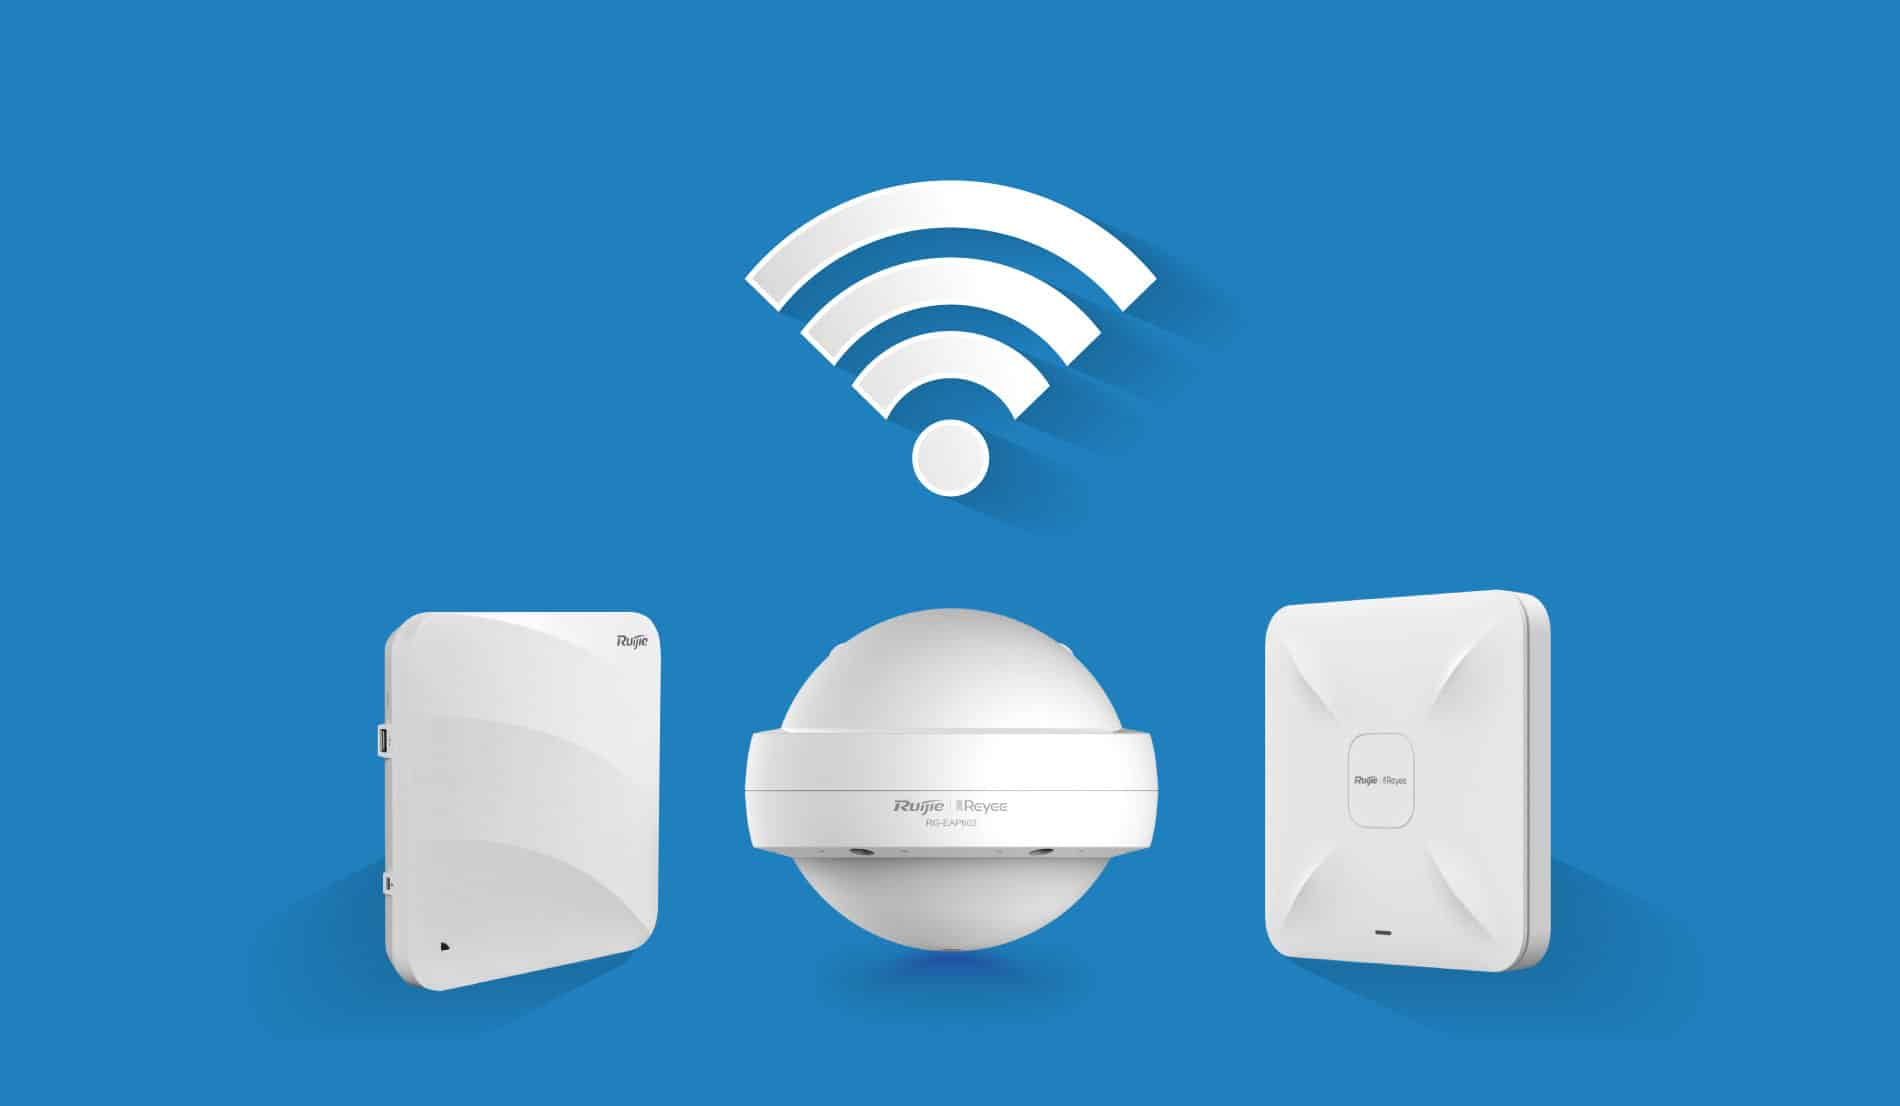
\includegraphics[width=0.85\textwidth]{2/figures/accesspoints.jpg}
		\caption[Access Points]{Access Points.\\
			Fuente: \cite{ot_cisco2024queesap}. \citetitle{ot_cisco2024queesap}.}
		\label{2:fig52}
	\end{center}
\end{figure}

Se pueden configurar para una variedad de funciones según nuestras necesidades. Algunas de las características incluyen:

\begin{itemize}
	\item \textbf{Modo cliente}: Se utiliza como receptor y se conecta a una red como un cable de red. \parencite{ot_ymant2023ap}
	\item \textbf{Modo AP (punto de Acceso)}: El punto de acceso es donde se instala el cableado y permite que varios usuarios accedan a la red. \parencite{ot_ymant2023ap}
	\item \textbf{Modo Repetidor}: Este modo puede extender la señal para que el punto de acceso amplifique la señal que recibe para maximizar el rango de acción. \parencite{ot_ymant2023ap}
	\item \textbf{Modo Bridge}: Este método se emplea para cubrir distancias considerables, como dos edificios distintos. Podemos establecer una red Wi-Fi a distancias significativas si conectamos dos puntos de acceso entre sí. \parencite{ot_ymant2023ap}
\end{itemize}

Los WAP son una opción más conveniente, segura y económica que los cables para conectar cada computadora o dispositivo a la red. Las empresas pequeñas pueden obtener muchas ventajas del uso de WAP para establecer una red inalámbrica. En primer lugar, las redes inalámbricas facilitan el acceso. Además, agregar nuevos usuarios es mucho menos difícil. Un invitado puede acceder fácilmente a Internet con una contraseña segura para la red inalámbrica. Además, se puede dividir fácilmente a los usuarios, incluidos los invitados, para proteger los recursos y activos de red. \parencite{ot_cisco2024queesap}

\begin{figure}[!ht]
	\begin{center}
		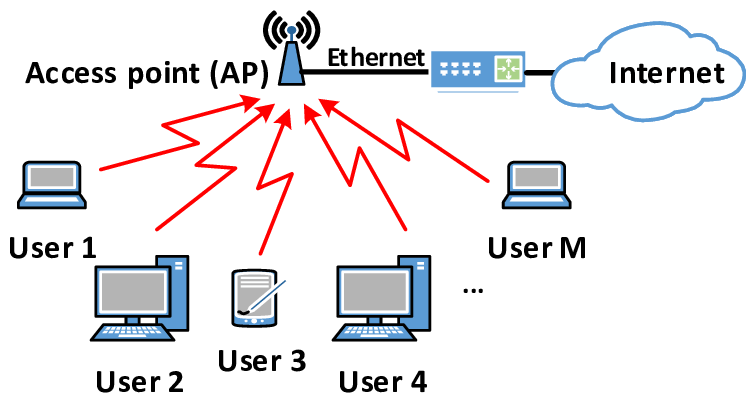
\includegraphics[width=0.85\textwidth]{2/figures/funcionap.png}
		\caption[Funcionamiento de un AP]{Funcionamiento de un AP.\\
			Fuente: \cite{ot_ymant2023ap}. \citetitle{ot_ymant2023ap}.}
		\label{2:fig53}
	\end{center}
\end{figure}

